% ns-3 ilk rapor (1 sayfa). Derleme: tectonic -X compile ns3_first_report.tex  (fontlar\ klasoru gerekir)
\documentclass[10pt,a4paper]{article}
\usepackage{fontspec}
\setmainfont{georgia}[Path=./fontlar/,Extension=.ttf,BoldFont=georgiab,ItalicFont=georgiai,BoldItalicFont=georgiaz]
\setsansfont{arial}[Path=./fontlar/,Extension=.ttf,BoldFont=arialbd,ItalicFont=ariali,BoldItalicFont=arialbi]
\setmonofont{consola}[Path=./fontlar/,Extension=.ttf,BoldFont=consolab,ItalicFont=consolai,BoldItalicFont=consolaz,Scale=0.88]
\usepackage[a4paper,left=2cm,right=2cm,top=1.6cm,bottom=1.4cm]{geometry}
\usepackage{xcolor,graphicx,titlesec,enumitem,amsmath}
\emergencystretch=3em
\definecolor{ink}{HTML}{1F2937}\definecolor{acc}{HTML}{1D4ED8}
\color{ink}
\titleformat{\section}{\sffamily\bfseries\large\color{acc}}{}{0pt}{}
\titlespacing*{\section}{0pt}{7pt}{3pt}
\setlength{\parindent}{0pt}\setlength{\parskip}{3pt plus 1pt}
\pagestyle{empty}
\begin{document}
{\sffamily\bfseries\Large ns-3 + 5G-LENA: Kurulum ve Çalıştırma}

\section*{1. Kurulum}
ns-3'ü Windows üzerinde çalıştırmak için WSL2 ve Ubuntu 24.04.5 LTS kurdum. Ubuntu içinde CMake 3.28.3 ve g++ 13.3.0 kullandım. ns-3.48 sürümünü \texttt{\textasciitilde/ehb415/ns-3-dev} klasörüne indirdim; 5G modülü olan 5G-LENA'yı (\texttt{contrib/nr}, etiket v5.1) ns-3.48 ile uyumlu sürüm olarak ekledim. Sürümleri birbirine kilitli seçmek gerekiyor (ns-3.48 $\leftrightarrow$ 5G-LENA v5.1). Derlemeyi \texttt{./ns3} aracıyla yaptım.

\section*{2. 5G-LENA demosunu çalıştırma}
Kurulumun çalıştığını görmek için 5G-LENA'nın hazır örneği \texttt{cttc-nr-demo}'yu 2 kullanıcıyla (UE) 1 saniyelik simülasyon olarak çalıştırdım (aşağıda akış sonuçları):

\medskip
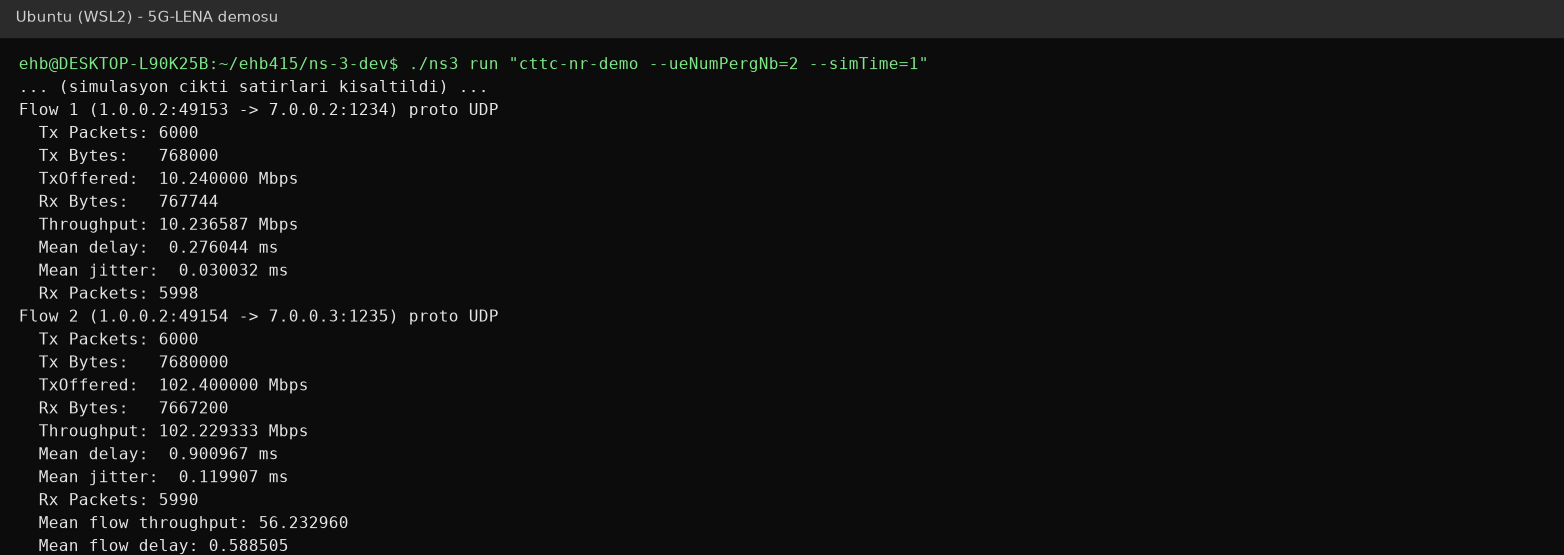
\includegraphics[width=\textwidth]{sekiller/ns3_rapor_demo.png}
\medskip

Çıktıda iki trafik akışı var. İlk akış 10,24\,Mbps gönderiliyor ve 10,24\,Mbps alınıyor, gecikme 0,28\,ms. İkinci akış 102,4\,Mbps gönderiliyor, 102,2\,Mbps alınıyor, gecikme 0,90\,ms. Alınan veri gönderilene çok yakın (kayıp \%0,03 ve \%0,17). Son satırdaki \textbf{Mean flow throughput 56,23\,Mbps} iki akışın ortalaması: $(10{,}24+102{,}23)/2=56{,}23$. Bu, 5G-LENA modülünün yüklendiğini ve simülasyonun sonuç ürettiğini gösteriyor.

\section*{3. Kendi yazdığım basit uygulama}
ns-3'ün nasıl çalıştığını anlamak için iki bilgisayar ve aralarında bir kablodan oluşan bir program yazdım (\texttt{scratch/benim\_ilk.cc}): kablo 5\,Mbps hızında ve 500\,ms gecikmeli, istemci 1024 baytlık tek bir paket yolluyor, sunucu bunu alıp geri cevap veriyor.

\medskip
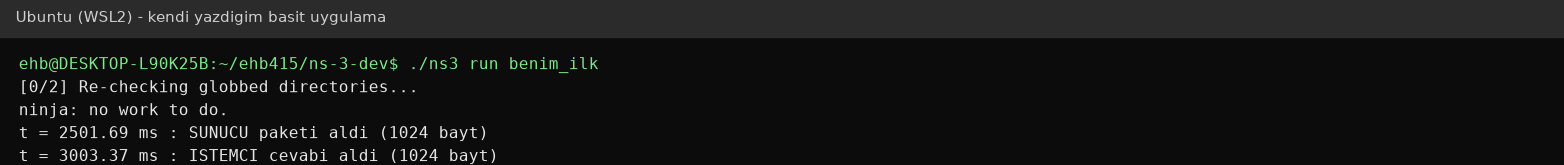
\includegraphics[width=\textwidth]{sekiller/ns3_rapor_ilk.png}
\medskip

Sonucu elle de hesapladım. Paket başlıklarıyla birlikte 1054 bayt: $1054\times 8/5\,\text{Mbps}=1{,}69$\,ms gönderme süresi, üstüne 500\,ms kablo gecikmesi = 501,69\,ms. İstemci t\,=\,2\,s'de gönderdiği için sunucu paketi t\,=\,2501,69\,ms'de aldı; cevap aynı yoldan döndüğü için istemci t\,=\,3003,37\,ms'de cevabı aldı. Simülasyon çıktısı elle hesapla birebir tuttu.

\section*{4. Değerlendirme}
Bu çıktılarla ns-3 ve 5G-LENA'nın kurulduğunu, derlenip çalıştığını ve sonuç ürettiğini doğruladım. Hazır 5G örneğinde veri kaybı çok düşük ve gecikme 1\,ms altında çıktı; yük kapasitenin altında olduğu için bu beklenen bir sonuç. Dikkat edilecek iki nokta var: (i) derleme profili ``optimized'' olduğu için \texttt{NS\_LOG} mesajları kapalı, sonuçları trace ve akış izleyicisi (FlowMonitor) çıktılarından okuyoruz; (ii) 5G-LENA'da hazır bir sensing modeli yok, bu yüzden projede ns-3 yalnızca haberleşme tarafının (throughput ve gecikme) maliyetini ölçecek.
\end{document}
